\documentclass{jlreq}

\usepackage{amsmath}
\usepackage{array}
\usepackage{bm}
\usepackage{caption}
\usepackage{fancyhdr}
\usepackage{float}
\usepackage{graphicx}
\usepackage{listings}
\usepackage{multirow}
\usepackage{physics}
\usepackage{siunitx}
\usepackage{xcolor}

\lstset{
    language=Python, % 使用するプログラム言語を指定
    basicstyle=\ttfamily\footnotesize, % フォントの指定
    numbers=left, % 行番号を表示(必要な場合)
    numberstyle=\tiny, % 行番号のスタイル
    frame=single, % ソースコードを枠で囲む(必要な場合)
    breaklines=true, % 長い行を自動的に折り返す
    captionpos=b, % キャプションの位置を下にする
    showstringspaces=false, % 文字列内のスペースを表示しない
    keywordstyle=\color{blue}, % キーワードの色
    commentstyle=\color{green}, % コメントの色
    stringstyle=\color{red}, % 文字列の色
}
\renewcommand{\lstlistingname}{ソースコード}

\numberwithin{equation}{section}

\pagestyle{fancy}
\fancyhf{}
\fancyhead[R]{\thepage}

\begin{document}

\tableofcontents
\clearpage

\section{目的}
学習データをもとに最近傍決定則や統計的識別で識別部を実装し,入力データを識別する.
また,識別部の性能評価を行い性能が信用できるかの考察を行う.

\section{実験手順}
\subsection{識別部の実装}
\subsubsection*{最近傍決定則}
\begin{enumerate}
  \item 学習データのそれぞれのクラスの平均ベクトルをプロトタイプ(お手本)として設定した
  \item 入力と最も近いプロトタイプを探索することで識別を行った
\end{enumerate}

\subsubsection*{統計的識別}
\begin{enumerate}
  \item 識別に必要な事前確率であるクラス$\omega_i$の生起確率と計算に必要なクラスの平均ベクトルと分散ベクトルを求めた
  \item ナイーブベイズ法を用いて,事前確率と各次元のクラス分布の値の積が最大となるクラスを識別結果とした
\end{enumerate}

\subsection{識別部の性能評価}

\section{結果}
学習データは配布された数字のデータを用いており,識別に最も適した特徴として縦横の分散を採用した.
\subsection{識別部の実装}
\subsubsection*{最近傍決定則}
最近傍決定則での識別部の実装をソースコード\ref{src:nearest}に示す.以下のコードでは,識別が正しく行われなかった入力に対してのみ出力するようにしている.
また,各クラスのプロトタイプとして,クラスの平均ベクトルを採用した.

\begin{lstlisting}[caption={最近傍決定則での識別部の実装}, label=src:nearest]
  from google.colab import drive
  drive.mount('/content/drive')
  
  import csv
  import matplotlib.pyplot as plt
  import numpy as np
  import pprint
  import random
  
  # クラス数
  NUM_CLASS = 10
  # クラスごとのデータ数
  NUM_CLASS_DATA = 10
  
  # 数字ラベル
  LABEL = 0
  # 重心
  MUX = 1
  MUY = 2
  # 分散
  VX = 3
  VY = 4
  # ゆがみ
  SX = 5
  SY = 6
  # 扁平度
  FX = 7
  FY = 8
  
  # CSV形式のファイルを行列に読み込み
  def read_csv(filename):
      with open(filename) as f:
          reader = csv.reader(f)
          data = list(reader)
      # 数値に変換
      data = [[float(value) for value in row] for row in data]
      return data
  
  # データを読み込む
  data = read_csv('/content/drive/MyDrive/pattern/week01/feature.csv')
  
  # Numpy操作用に変換
  data = np.array(data)
  
  # 各クラスの平均ベクトルを求める関数
  def get_class_mean(feature_list):
    res = np.empty((0, 9))
  
    for i in range(NUM_CLASS):
      start = i * NUM_CLASS
      mean_vec = np.mean(feature_list[start : start + NUM_CLASS_DATA], axis=0)
      res = np.append(res, [mean_vec], axis=0)
  
    return res
  
  # 各クラスのプロトタイプ(今回は平均ベクトルをプロトタイプとした)
  prototype_list = get_class_mean(data)
  # print(prototype_list)
  
  #===============================================================================
  #                                最近傍決定則
  #===============================================================================
  
  # 特徴ベクトルf1とf2の距離を求める関数
  def get_distance(f1, f2, idx1, idx2):
    p = np.array([f1[idx1], f1[idx2]])
    q = np.array([f2[idx1], f2[idx2]])
    return np.linalg.norm(p - q)
  
  # 特徴の組み合わせ(idx1, idx2)に対して,識別を行う関数
  def recognize_by_nn(feature, idx1, idx2):
    l = []
  
    for i in range(NUM_CLASS):
      dist = get_distance(feature, prototype_list[i], idx1, idx2)
      l.append(dist)
  
    return l.index(min(l))
  
  #===============================================================================
  #                                   入力と実行
  #===============================================================================
  
  for i in range(NUM_CLASS):
    for j in range(NUM_CLASS_DATA):
      feature = data[i * NUM_CLASS + j]
      result = recognize_by_nn(feature, VX, VY)
      if i != result:
        print('target number: ' + str(i))
        print('case number: ' + str(j))
        print('result: ' + str(result) + '(' + str(i == result) + ')')
        print('')
\end{lstlisting}

出力結果を図\ref{fig:result_nearest}に示す.
\begin{figure}[H]
  \centering
  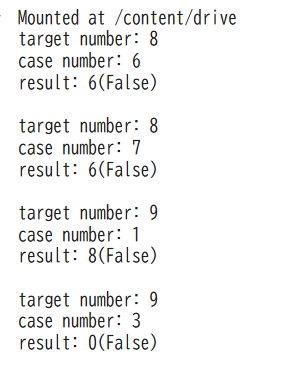
\includegraphics{image/nearest_result.png}
  \caption{最近傍決定則での出力結果}
  \label{fig:result_nearest}
\end{figure}

最近傍決定則の精度は$1 - \frac{4}{100} = 0.96$,つまり$96\si{\percent}$であった.

\subsubsection*{統計的識別}
ナイーブベイズ法による識別部の実装をソースコードに示す.以下のコードにおいても,識別が正しく行われなかった入力に対してのみ出力するようにしている.

\begin{lstlisting}[caption={ナイーブベイズ法による識別部の実装}, label=src:naive]
  from google.colab import drive
  drive.mount('/content/drive')
  
  import csv
  import matplotlib.pyplot as plt
  import numpy as np
  import statistics
  import math
  
  # クラス数
  NUM_CLASS = 10
  # クラスごとのデータ数
  NUM_CLASS_DATA = 10
  
  # 数字ラベル
  LABEL = 0
  # 重心
  MUX = 1
  MUY = 2
  # 分散
  VX = 3
  VY = 4
  # ゆがみ
  SX = 5
  SY = 6
  # 扁平度
  FX = 7
  FY = 8
  
  # CSV形式のファイルを行列に読み込み
  def read_csv(filename):
      with open(filename) as f:
          reader = csv.reader(f)
          data = list(reader)
      # 数値に変換
      data = [[float(value) for value in row] for row in data]
      return data
  
  # データを読み込む
  data = read_csv('/content/drive/MyDrive/pattern/week01/feature.csv')
  
  # Numpy操作用に変換
  data = np.array(data)
  
  #===============================================================================
  #                               ナイーブベイズ
  #===============================================================================
  
  # 識別に適した特徴の組み合わせ
  IDX1 = VX
  IDX2 = VY
  
  # 各クラスの事前確率P(ωi)
  PRIOR_PROBABLITY = 0.1
  
  # 各クラスの平均ベクトルを求める関数
  def get_class_mean(feature_list):
    res = np.empty((0, 9))
  
    for i in range(NUM_CLASS):
      start = i * NUM_CLASS
      mean_vec = np.mean(feature_list[start : start + NUM_CLASS_DATA], axis=0)
      res = np.append(res, [mean_vec], axis=0)
  
    return res
  
  # 各クラスの分散を求める
  def get_class_variance(feature_list):
    res = np.empty((0, 9))
  
    for i in range(NUM_CLASS):
      start = i * NUM_CLASS
      var_vec = np.var(feature_list[start : start + NUM_CLASS_DATA], axis=0)
      res = np.append(res, [var_vec], axis=0)
  
    return res
  
  # 各クラスの平均ベクトル
  mean_list = get_class_mean(data)
  # 各クラスの分散
  variance_list = get_class_variance(data)
  
  # 正規分布関数
  def normal(x, u, v):
    res = 1 / np.sqrt(2 * np.pi * v) * np.exp(-(x-u)**2/(2*v))
    return res
  
  # 尤度を求める関数
  def get_likelihood(feature, mean, var):
    p1 = normal(feature[IDX1], mean[IDX1], var[IDX1])
    p2 = normal(feature[IDX2], mean[IDX2], var[IDX2])
    return p1 * p2
  
  def recognize_by_naive_bayes(vec_in):
    l = []
  
    for i in range(NUM_CLASS):
      p = PRIOR_PROBABLITY * get_likelihood(vec_in, mean_list[i], variance_list[i])
      l.append(p)
  
    return l.index(max(l))
  
  #===============================================================================
  #                                   入力と実行
  #===============================================================================
  
  for i in range(NUM_CLASS):
    for j in range(NUM_CLASS_DATA):
      feature = data[i * NUM_CLASS + j]
      result = recognize_by_naive_bayes(feature)
      if i != result:
        print('target number: ' + str(i))
        print('case number: ' + str(j))
        print('result: ' + str(result) + '(' + str(i == result) + ')')
        print('')
\end{lstlisting}

出力結果を図\ref{fig:result_naive}に示す.
\begin{figure}[H]
  \centering
  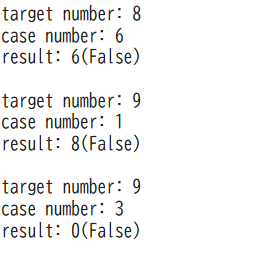
\includegraphics{image/naive_result.png}
  \caption{ナイーブベイズ法での出力結果}
  \label{fig:result_naive}
\end{figure}

ナイーブベイズ法の精度は$1 - \frac{3}{100} = 0.97$,つまり$97\si{\percent}$であった.

以上の結果から,最近傍決定則よりもナイーブベイズ法の方が識別の精度が高くなった.

\subsection{識別部の性能評価}

\section{考察}
\subsection{最近傍決定則と統計的識別の識別精度の違い}

\subsection{識別部の評価}

\begin{thebibliography}{9}
  \item 崔恩瀞.プロジェクト実習Ⅱ パターン認識 実験テキスト.京都工芸繊維大学,2024年
\end{thebibliography}

\end{document}